\section{Approach}
\label{approach}
% \subsection{Overview}

\begin{figure*}[t]
    \centering
    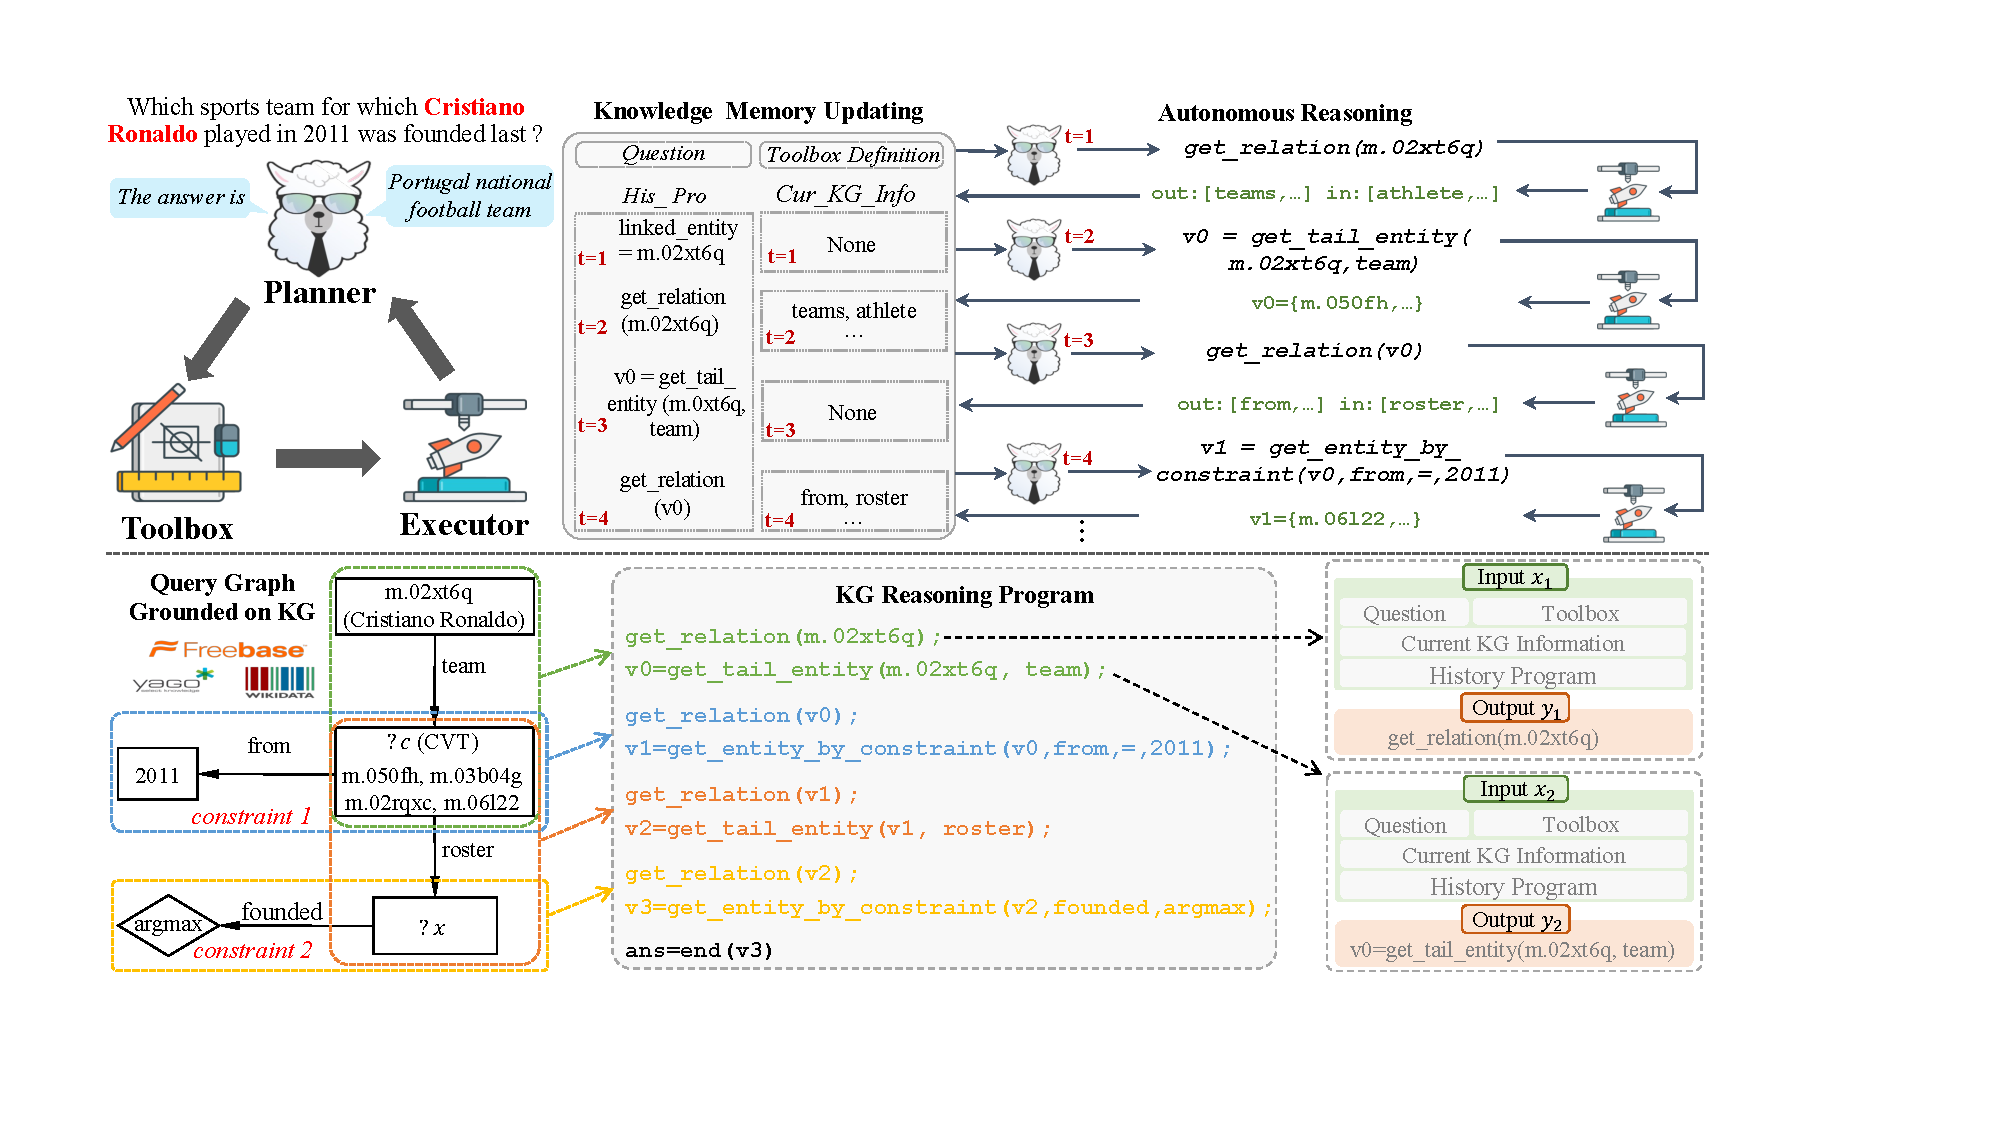
\includegraphics[width=2.1\columnwidth]{resource/model.pdf}
    \caption{The overview of our proposed KG-Agent. The top half is the workflow of our agent, and the bottom half is an example of instruction fine-tuning data synthesis and the prompt template for the input-output pairs. For brevity, we simplify the relation surface form.}
    \label{fig:model}
    % \vspace{-0.3cm}
\end{figure*}

In this part, we present the proposed \textbf{KG-Agent} for autonomously solving complex reasoning tasks over KG. The core of our KG-Agent framework is a well-instructed LLM, which can autonomously make decisions when reasoning over KG.
We first extend the LLM's capacities by designing a toolbox with supporting tools to manipulate the KG data or intermediate results (Section~\ref{sec:toolbox}). 
To enhance the step-by-step reasoning capacity, we leverage existing knowlege graph question answering~(KGQA) datasets to synthesize KG reasoning programs and convert them into formatted instruction tuning data (Section~\ref{sec:tuning}). Finally, we design an effective agent framework based on the knowledge memory to support autonomous reasoning over KG (Section~\ref{sec:utilization}).  
Next, we give the technical details of KG-Agent.  

\subsection{Toolbox for Knowledge Graph}
\label{sec:toolbox}
Since LLMs struggle to accurately manipulate the structured data~\cite{Jiang-2023-arxiv-StructGPT}, we construct a supporting toolbox for easing the utilization of the KG information.
According to existing work~\cite{GrailQA,KQA-Pro}, reasoning over KG ~(\eg Freebase or Wikidata) typically requires three fundamental operations, namely extracting information from KG, filtering irrelevant information based on the semantics of the question, and operating on the extracted information.
Therefore, we design three types of tools for LLMs reasoning over KG, \ie extraction, semantic, and logic tools.

$\bullet$ \textbf{Extraction tools} aim to facilitate the access to information from KG. 
%This type of tool aims to access the useful knowledge in KGs. 
Considering the basic data types in  KG, we design five tools to support the access to the relations (\emph{get\_relation}), the head/tail entities (\emph{get\_head\_entity}/\emph{get\_tail\_entity}), and entities with specific type or constraint (\emph{get\_entity\_by\_type}/ \emph{get\_entity\_by\_constraint}), \emph{w.r.t.} some entity set or other input information (\eg relation or type).  

$\bullet$ \textbf{Logic tools} aim to 
support basic manipulation operations on the extracted KG information, including entity counting (\emph{count}), entity set intersection (\emph{intersect}) and union (\emph{union}), condition verification (\emph{judge}), and ending the reasoning process with the current entity set as the final answer(s) (\emph{end}). 

$\bullet$ \textbf{Semantic tools}
are developed by utilizing pre-trained models to implement specific functions, including relation retrieval (\emph{retrieve\_relation}) and entity disambiguation (\emph{disambiguate\_entity}). 
These tools extend the basic operations on KGs and can support advanced functionalities for KG reasoning. 

We summarize the detailed definition and usage of the tools in Table~\ref{tab:toolbox} at the Appendix~\ref{sec:app-tool}. Note that since the format and usage for each tool have been defined in a unified way, the toolbox for KG can be flexibly extended according to the real needs.

\subsection{KG-Agent Instruction  Tuning}
\label{sec:tuning}
To enable the autonomous reasoning process, we construct a high-quality instruction dataset for fine-tuning a small LLM (\ie LLaMA2-7B).
For this purpose, we first leverage existing KG based question answering~(KGQA) datasets to generate the KG reasoning program, and then decompose it into multiple steps. Finally, each step is formulated as the instruction data with input and output.

\subsubsection{KG Reasoning Program Generation}\label{sec-KG-RPG}
Instead of distilling from close-sourced LLMs (\eg GPT-4),  we propose to leverage existing KGQA datasets to synthesize the KG reasoning program. 
These KGQA datasets contain the annotated SQL queries that can be executed to directly extract the answer entities for each question. 
In particular, the SQL query generally includes the relation chain, conditions, or constraints, which are beneficial for reasoning program synthesis.  
Concretely, we first ground the SQL query on the KG to obtain a query graph, then extract the reasoning chain and constraint conditions from the query graph, and finally decompose the chain into multiple code snippets as the reasoning program.


\paratitle{Reasoning Chain Extraction.}
Since the whole KG is extremely large and contains irrelevant data, the first step is to acquire a small KG subgraph related to the question, referred to as \emph{query graph}. Following previous work~\cite{Yin-acl-20}, we obtain the query graph from the KG via rule match.
As shown in Figure~\ref{fig:model}~(b), the query graph has a tree-like structure that can be directly mapped to a logical form~\cite{Yin-acl-20}, and it can clearly depict the execution flow of the SQL query to obtain the answer. 
Second, starting from the mentioned entity in the question (\ie \emph{Cristiano Ronaldo}), we adopt breadth-first search~(BFS) to visit all the nodes on the query graph. 
This strategy would finally produce a reasoning chain~(\eg \textit{teams$\rightarrow$roster\_team}) linking the start entity to the answer entity, and the relevant constraint conditions~(\eg \textit{roster\_from} $=$ ``2011'') or numerical operation~(\eg \textit{founded} must be last) can be naturally involved in this process. 

\paratitle{Reasoning Program Generation.} After extracting the reasoning chain, we next convert it into multiple interrelated triples, where each triple generally corresponds to an intermediate reasoning step.
Finally, we reformulate the triples into several function calls with the code format, which represents the tool invocation and can be executed to obtain the corresponding triples based on the KG.
Given a triple $\langle e, r, e'\rangle$, we craft a rule-based method to synthesize the function calls that represent the information flow from $e$ to $e'$.
Specifically, we start from the \emph{get\_relation(e)} function call to obtain the current candidate relations $\{r\}$ associated with $e$ on the KG. Then, we select one relation $r$ and pass it to other required function calls~(\eg \textit{get\_tail\_entity} or \textit{get\_entity\_by\_constraint}), and finally obtain new entities.
Following the order of the reasoning chain, we generate all the function calls to compose the final KG reasoning program for producing the instruction dataset.
We show one example in Figure~\ref{fig:model}~(b) to intuitively illustrate the conversion process from the annotated SQL query to our required KG reasoning program.

\subsubsection{KG Reasoning Instruction Synthesis}\label{sec-instruction-syn}
After obtaining the reasoning program on KG, we further utilize it for synthesizing instruction data for supervised fine-tuning (SFT).  
As discussed in Section~\ref{sec-KG-RPG}, our instruction data is highly based on the reasoning program, which is aligned with the intermediate reasoning steps for KGQA.  

\paratitle{Input-Output Pair Construction.}
The synthetic KG reasoning program consists of multiple function calls in a sequence. For each function call, we aim to construct an input-output pair as the instruction. Specifically, the input contains the question, toolbox definition, current KG information (\ie the next candidate relations of the current entity set), and history reasoning program before the current step; and the output is the function call at the current step.
Next, after executing the function call at the current reasoning step, the history reasoning program and current KG information in the input will be accordingly updated, and the output will be updated as the function call at the next step.
By iterating the above process, for each sample in the KGQA datasets, we can obtain multiple input-output pairs derived from the corresponding reasoning program, which depict the complete reasoning trajectory on the KG.
To help LLMs better understand, we further utilize a unified prompt, as shown in Figure~\ref{fig:model}~(c), to format each input-output pair and obtain the final instruction tuning data.

\paratitle{Agent Instruction Tuning.}
Based on the above formatted instruction tuning data, we perform supervised fine-tuning on a small LLM~(\ie LLaMA-7B), which is much smaller than the backbone models in previous work~\cite{Jiang-2023-arxiv-StructGPT}.
Formally, for each sample, we formulate all input-output pairs of the complete trajectory in the format of $\{\langle x_1, y_1 \rangle , ..., \langle x_t, y_t \rangle, ..., \langle x_{n}, y_{n} \rangle \}$, where $\langle x_t, y_t \rangle$ represent the input and ground-truth response in the $t$-th step and $n$ represents the total steps.
For simplicity, we denote each input and output as $x$ and $y$ below.
During the instruction tuning process, we feed the input~$x$ and output~$y$ into the decoder-only LLM and minimize the cross-entropy loss on the ground-truth response~$y$ as:
\begin{align}
    \mathcal{L} = - \sum_{k=1}^m \log \text{Pr}(y_k|x, y_{<k}),
\end{align}
where $m$ denotes the number of tokens in $y$, $y_k$ and $y_{<k}$ are the $k$-th and previous tokens in the output.

\begin{table}[t]
        \renewcommand\arraystretch{1.0}
        \setlength\tabcolsep{2.5pt}
	\centering
	\small
            \begin{tabular}{l |  c | c c c c }
			\toprule
			\textbf{Method} & \textbf{\makecell{Work\\ Flow}} & \textbf{\makecell{Base \\Model}} & \textbf{Tool} & \textbf{Memory} & \textbf{\makecell{Multi\\Task}} \\
			\midrule
			Pangu & pd & T5-3B & \xmark & \xmark & \xmark\\
                StructGPT & pd & ChatGPT  & \cmark  & \xmark & \xmark\\
			RoG & pd & LLaMA-7B & \xmark & \xmark & \xmark\\
                ChatDB & auto & ChatGPT & \xmark & \cmark & \xmark\\
                KB-BINDER & pd & CodeX & \xmark & \xmark & \xmark\\
                \midrule
                KG-Agent & auto & LLaMA2-7B & \cmark & \cmark & \cmark\\
    		\bottomrule
		\end{tabular}
        \caption{Comparison of different methods. \textbf{\emph{Work Flow}} describes that the interaction way between the LLM and KG is pre-defined~(``pd'') or autonomous~(``auto''). \textbf{\emph{Multi Task}} means whether to support generalization across different KGs via multi-task learning.}
	\label{tab:res}
    \vspace{-0.3cm}
\end{table}

\subsection{Autonomous Reasoning over KG}
\label{sec:utilization}
After instruction tuning, we further design an effective agent framework
that enables KG-Agent to autonomously perform multi-step reasoning over KG for answer finding.
The overall illustration of KG-Agent is shown in Figure~\ref{fig:model}~(a).
It mainly contains four components, \ie the core instruction-tuned LLM (Section~\ref{sec:tuning}), referred to as the \emph{LLM-based planner}, the multifunctional \emph{toolbox}~(Section~\ref{sec:toolbox}), the \emph{KG-based executor} for executing the tool invocation, and the \emph{knowledge memory} to record the context and currently useful information in the whole process.
Next, we introduce how KG-Agent performs autonomous reasoning over KG.

\paratitle{Knolwedge Memory Initialization.}
The knowledge memory preserves the currently useful information to support the LLM-based planner for making decisions.
It mainly contains four parts of information, \ie natural language question, toolbox definition, current KG information, and history reasoning program.
The former two parts are initialized with the given question and toolbox definition, which remain unchanged during the reasoning process.
The later two parts are initialized as an empty list, which will be constantly updated at each step after LLM generating the function call and executor invoking the corresponding tool.

\paratitle{Planner for Tool Selection.}
Based on the current knowledge memory, the LLM-based planner selects a tool to interact with KG at each step.
Specifically, all the parts in the current knowledge memory will be formatted with corresponding prompt template to compose the input (used in Agent Instruction Tuning in Section~\ref{sec-instruction-syn}), and then the LLM will generate one function call by selecting a tool and its arguments from the input. 
Generally, the planner needs to invoke tools from the pre-defined toolbox to address four types of task requirements, \ie linking the mentioned entity to KG (\eg ``\emph{get\_candidate\_entity}'' and ``\emph{disambiguate\_entity}''), accessing the KG information (\eg \textit{``get\_relation''} and \textit{``get\_head\_entity''}), processing the intermediate results (\eg \textit{``count''} and \textit{``intersect''}), or returning the final answer to end the reasoning process (\eg \textit{``end''}).


\begin{table*}
\small
\centering
\resizebox{\textwidth}{!}{\begin{tabular*}{\textwidth}{l@{\extracolsep{\fill}}cccccccc}
\toprule
\multirow{2.5}{*}{\textbf{Model}}& \multicolumn{2}{c}{\textbf{WebQSP}}   &\multicolumn{2}{c}{\textbf{CWQ}} &\multicolumn{4}{c}{\textbf{GrailQA~(F1)}} \\ 
\cmidrule{2-3}\cmidrule{4-5}\cmidrule{6-9}
& \textbf{Hits@1} & \textbf{F1} & \textbf{Hits@1} & \textbf{F1} & \textbf{Overall} &  \textbf{I.I.D.} & \textbf{Compositional} & \textbf{Zero-shot}  \\
\midrule
GraftNet     & 66.4  &  60.4     & 36.8  & 32.7      & - &   -    & -  &  -   \\
NSM      & 68.7  &  62.8     & 47.6  & 42.4    & -   & -    & -  &  -   \\
SubgraphRetrieval   & 69.5& 64.1  & 49.3& 46.3 &  - & - & -  &  -   \\
UniKGQA      &  75.1& 70.2  & 50.7 & 48.0 &  - & -    & -  &  -  \\
ReasoningLM &  78.5& 71.0  & 69.0 & 64.9 &  - & -    & -  &  -  \\
\midrule
RNG-KBQA    & -  &  75.6     & -  & -    & 76.8  &   89.0    & 68.9  &  74.7   \\
Uni-Parser & -  &  75.8     & -  & -    & 76.5  &   88.3    & 71.4  &  73.4   \\
ArcaneQA & - &75.6 & -  & -       & 76.9  &   89.2    & 73.9  &  72.8 \\
PanGu w/ T5-3B & - & 79.6 & - & - & 83.4 & - & - & - \\
TIARA & 75.2 & 78.9 & -  & -       &  81.9  &   91.2    & 74.8  &  80.7 \\
FC-KBQA & - & 76.9 & - & 56.4 & 83.8 & 91.5 & 77.3 &  83.1 \\
\midrule
ROG & \textbf{85.7} & 70.8 & 62.6 & 56.2 & -  & - & - & - \\
ChatGPT & 67.4 & 59.3 & 47.5 & 43.2 & 25.3 & 19.6 & 17.0 & 31.2 \\
Davinci-003 & 70.8 & 63.9 & 51.4 & 47.6 & 30.1 & 23.5 & 22.0 & 36.4 \\
GPT-4 & 73.2 & 62.3 & 55.6 & 49.9 & 31.7 & 25.0 & 20.6 & 39.2 \\
StructGPT & 72.6 & 63.7 & 54.3 & 49.6 & 54.6 & 70.4 & 44.3 & 50.5 \\
\midrule
\multicolumn{1}{l}{Ours} & 83.3 & \textbf{81.0}  & \textbf{72.2} & \textbf{69.8} & \textbf{86.1} & \textbf{92.0} & \textbf{80.0} & \textbf{86.3} \\
\bottomrule
\end{tabular*}}
\caption{The results on the test set of WebQSP and CWQ, and dev set of GrailQA, which are based on Freebase KG. We copy part of the results from~\citet{Jiang-2023-arxiv-StructGPT,Gu-ACL-23,Luo-arxiv-23-Reasoning} and evaluate ChatGPT,Davinci-003, GPT-4, and StructGPT with OpenAI API. Bold font denotes the best performance.}
\label{tab:fb-res}
\end{table*}

\paratitle{Executor for Memory Updation.}
After the planner generates the function call, the KG-based executor will execute it using a program compiler. It can cache or operate the intermediate variables, and extract new entities or relations from the KG. After execution, the knowledge memory will be accordingly updated. First, the current function call will be added to the history reasoning program. Second, if the invoked tool is to obtain the new information from the KG (\eg ``\emph{get\_relation}''), 
the executor will add it to the KG information for updating the knowledge memory.

\paratitle{Iterative Autonomous KG-Agent.}
The KG-Agent framework autonomously iterates the above tool selection and memory updation process to perform step-by-step reasoning, where the knowledge memory is used to maintain the accessed information from KG. 
In this way, the multi-turn decision-making process of the agent is like walking on the KG along relations.
Once reaching the answer entities, the agent will automatically stop the iterative process.
Note that the whole process is agnostic to the task types (\eg question answering) and some specific KGs. Therefore, our approach is a general framework that can be applied to a variety of complex tasks that require reasoning over any KGs.

% \paratitle{Differences with Previous Work}.
\subsection{Comparison to Previous Work}

% \paratitle{Comparison to Previous Work.} 
Existing methods of reasoning over KG can be categorized into two classes based on their workflow. The first line of research, such as KB-BINDER~\cite{Li-ICLKBQA-arXiv-23}, Pangu~\cite{Gu-ACL-23}, StructGPT~\cite{Jiang-2023-arxiv-StructGPT}, and RoG~\cite{Luo-arxiv-23-Reasoning}, crafted a pre-defined interaction way between LLM and KG, which cannot flexibly adapt to various complex tasks. Another line of research, such as ChatBD~\cite{ChatDB}, conducted autonomous reasoning with chain-of-thought and memory augmented. However, it relies on the strong closed-source LLM APIs~(\eg ChatGPT) and cannot use tools to implement some specialized operations~(\eg count). Our KG-Agent is the first autonomous agent framework to support the complex interaction between LLM and KG with tool and memory augmented. Furthermore, we implement this autonomous agent by instruction tuning a smaller 7B open-source LLM compared to the backbone LLM in KB-BINDER, StructGPT, and ChatDB.
At the same time, the agent instruction tuning data is constructed from various KGs~(\eg Wikidata and Freebase), which helps our KG-Agent to learn the general autonomous decision making capabilities over various KGs.